\par\vspace{2mm}
Les forces en présence sont la gravité
\begin{align}
    m\bm g &= mg\sin(\alpha) \ex - mg\cos(\alpha) \ey
\end{align}
et la force de soutient normale au câble
\begin{align}
    \bm N  = N \bm e_y.
\end{align}

Le théorème du centre de masse stipule que l'on peut appliquer la seconde loi de Newton en considérant chaque force appliquée sur la barre au centre de masse G.
On obtient alors 
\begin{align}
    m \bm a_G &= \sum \bm F \nonumber\\
    \Leftrightarrow m (\bm a'_G + \bm a_A) &= m\bm g + \bm N \label{eq:newtonCM}
\end{align}
o\`u $\bm a_G$ est l'accélération du centre de masse selon le référentiel d'inertie lié à $O$ et $\bm a'_G$ selon le référentiel accéléré lié à $A$. $\bm a_A$ est l'accélération relative du référentiel lié en $A$ par rapport au référentiel d'inertie.
En utilisant le repère cartésien $(\ex,\ey)$, on écrit la $\overrightarrow{OA}=x_A \ex$ et donc l'accélération $\bm a_A$ s'écrit
\begin{equation}
    \bm a_A = \frac{\mathrm d^2}{\mathrm dt^2}\overrightarrow{OA}= \ddot x_A \ex.
\end{equation}
D'une manière similaire, l'accélération relative du centre de masse $\bm a'_G$ peut s'obtenir en dérivant deux fois la position du centre de masse dans le repère $(\ex,\ey)$, i.e. $\overrightarrow{AG}=l\sin(\theta)\ex-l\cos(\theta)\ey$.
\begin{align}
    \bm a'_G &= \frac{\mathrm d^2}{\mathrm dt^2}\overrightarrow{AG}\nonumber\\
    &= \frac{\mathrm d}{\mathrm dt}\left[l\cos(\theta)\dot\theta \ex + l\sin(\theta)\dot\theta \ey \right]\nonumber\\
    &= \left[l\cos(\theta)\ddot\theta  - l\sin(\theta)\dot\theta^2 \right]\ex +  \left[l\sin(\theta)\ddot\theta + l\cos(\theta)\dot\theta^2\right]\ey
\end{align}
Ainsi, l'équation Eq. \eqref{eq:newtonCM} se développe selon $\ex$ et $\ey$ en
\begin{align}
ml\ddot\theta\cos(\theta) - ml\dot\theta^2 \sin(\theta)  + m\ddot x_A &= m g \sin(\alpha)\label{eq:newton_ex}\\
ml\ddot\theta\sin(\theta) +ml \dot\theta^2\cos(\theta) &= N - mg\cos(\alpha) \label{eq:newton_ey}.
\end{align}

 \begin{figure}
     \centering
     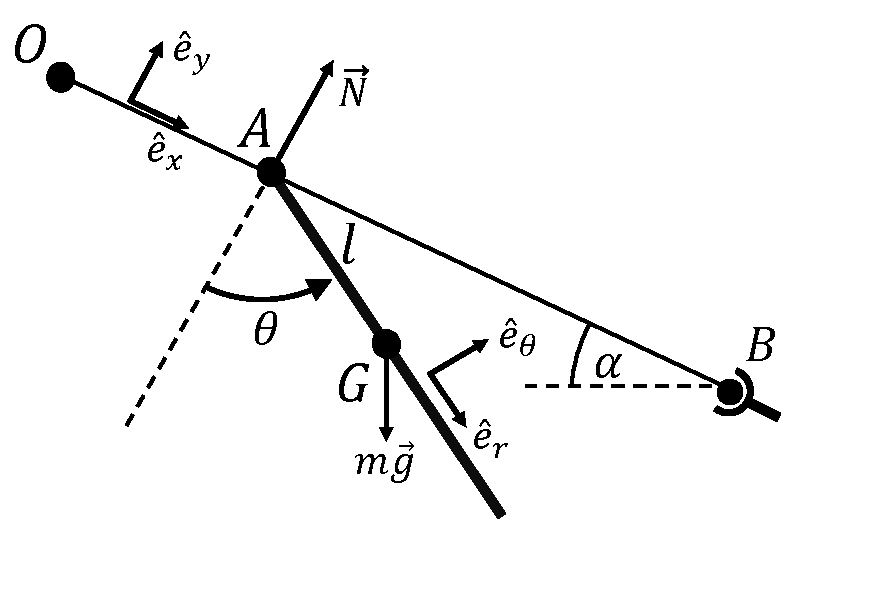
\includegraphics[width=0.5\linewidth]{ExoFig/tyr_schema_details.pdf}
     \caption{Schéma détaillé du problème}
     \label{fig:schema_details}
 \end{figure}